\documentclass[a4paper,12pt]{report}
\usepackage{graphicx}
\usepackage{hyperref}
\usepackage[T1]{fontenc}
\usepackage[utf8]{inputenc}
\usepackage{array}
\usepackage{setspace}
\usepackage[paper=a4paper,margin=1in]{geometry}


\begin{document}
    
    \begin{titlepage}
        
        \noindent
        \begin{minipage}[t]{0.19\textwidth}
            \vspace{-4mm}{
\includegraphics[scale=1.15]{image/logo-unimib.pdf}}
        \end{minipage}
        \begin{minipage}[t]{0.81\textwidth}
        {
                \setstretch{1.42}
                {\textsc{Università degli Studi di Milano - Bicocca}} \\
                \textbf{Scuola di Scienze} \\
                \textbf{Dipartimento di Informatica, Sistemistica e Comunicazione} \\
                \textbf{Corso di laurea in Informatica} \\
                \par
        }
        \end{minipage}
        
	\vspace{55mm}
        
	\begin{center}
            {\LARGE{
                    \setstretch{1.2}
                    \textbf{Relazione Finale del Progetto d'Esame\\ del corso di Ingegneria del Software \\ Brew-Day! }
                    \par
            }}
        \end{center}
        
        \vspace{50mm}
  

        \begin{flushright}
            {\large \textbf{Componenti del gruppo:}} \\
            \large{Gilardi Alessandro - 866035} \\
            \large{Refolli Francesco - 865955} \\
            \large{Qazim Toska - 847361} \\
        \end{flushright}
        
        \vspace{40mm}
        \begin{center}
            {\large{\bf Anno Accademico 2022-2023}}
        \end{center}

        \restoregeometry
        
    \end{titlepage}
    
    \newpage
   \tableofcontents
   
   \newpage
    
    
    \chapter{Introduzione}
	Questa è una breve introduzione all'applicazione
	
    \chapter{Analisi}
    	\section{Glossario}
    		\begin{table}[!h]
      			\renewcommand{\arraystretch}{1.2}
      			\begin{tabular}{p{0.2\textwidth}|p{0.7\textwidth}} 
        				\textbf{Nome}  & \textbf{Descrizione} \\
    				\hline
           			birraio & un utente \\
                        		equipaggiamento & bollitore, fermentatore, pipa da birra \\
                            	capacita' & quantita' in litri che un equipaggiamento puo' supportare in una turnata \\
                          	ingrediente & malto, luppolo, lievito, zucchero, acqua, additivi \\
                          	ricetta & collezione di ingredienti con associata una quantita' \\
                          	inventario & collezione di ingredienti che l'home brewer ha a disposizione \\
                            	consiglio & ricetta che massimizza l'uso degli ingredienti nell'inventario \\
                            	istanza di birra & anche chiamata `istanza di ricetta` nel testo, birra prodotta con una certa ricetta \\
        			\end{tabular}
        			\caption{Glossario}
      			\label{tab:Gloassario}
    		\end{table}
	
    \newpage
	\section{Requisiti Funzionali}
	
    		\begin{table}[!h]
      			\renewcommand{\arraystretch}{1.2}
      			\begin{tabular}{p{0.8\textwidth}|p{0.1\textwidth}} 
        				\textbf{Requisito}  & \textbf{MoSCoW} \\
    				\hline
                                  il sistema deve permettere all'utente di mantenere, aggiornare, eliminare ricette & M \\
                                  il sistema deve permettere all'utente di mantenere l'inventario & M \\
                                  il sistema deve permettere all'utente di indicare che una ricetta e' stata eseguita e quindi aggiornare l'inventario di conseguenza & M \\
                                  il sistema deve permettere all'utente di indicare che ha fatto la spesa e quindi aggiornare l'inventario di conseguenza & M \\
                                  il sistema deve permettere all'utente di produrre la lista della spesa per gli ingredienti mancanti di una ricetta & M \\
                                  il sistema deve permettere all'utente di generare un consiglio per la prossima birra & M \\
                                  il sistema deve permettere all'utente di mantenere le istanze di una ricetta & M \\
                                  il sistema deve permettere all'utente di aggiungere, aggiornare, eliminare note alle istanze di una birra & M \\
                                  il sistema deve notificare l'utente quando mancano degli ingredienti per la prossima birra & M \\
        			\end{tabular}
        			\caption{Requisiti Funzionali}
      			\label{tab:Requisiti Funzionali}
    		\end{table}
	
	
	
	\section{Specifiche Supplementari}
	
    		\begin{table}[!h]
      			\renewcommand{\arraystretch}{1.2}
      			\begin{tabular}{p{0.8\textwidth}|p{0.1\textwidth}} 
        				\textbf{Requisito}  & \textbf{MoSCoW} \\
    				\hline
                                  il sistema deve mantenere le quantita' degli ingredienti nelle ricette (e nell'inventario) in termini di unita' assolute (anche diverse), in modo che sia piu' semplice calcolare i multipli & M \\
                                  il sistema deve supportare le note normale e le note di sapore per le istanze di una ricetta  & M \\
                                  il suggerimento della birra deve massimizzare l'uso di ingredienti e equipaggiamento & M \\
                                  il sistema deve supportare la possibilita' di aggiungere immagini alle istanze di birra & C \\
                                  si deve permettere di eliminare una ricetta che ha associate delle birre prodotte & M \\
        			\end{tabular}
        			\caption{Specifiche Supplementari}
      			\label{tab:Specifiche Supplementari}
    		\end{table}	
	
	
    \newpage
	\section{Casi d'Uso}
	
		\begin{figure}[!h]
			\centering
			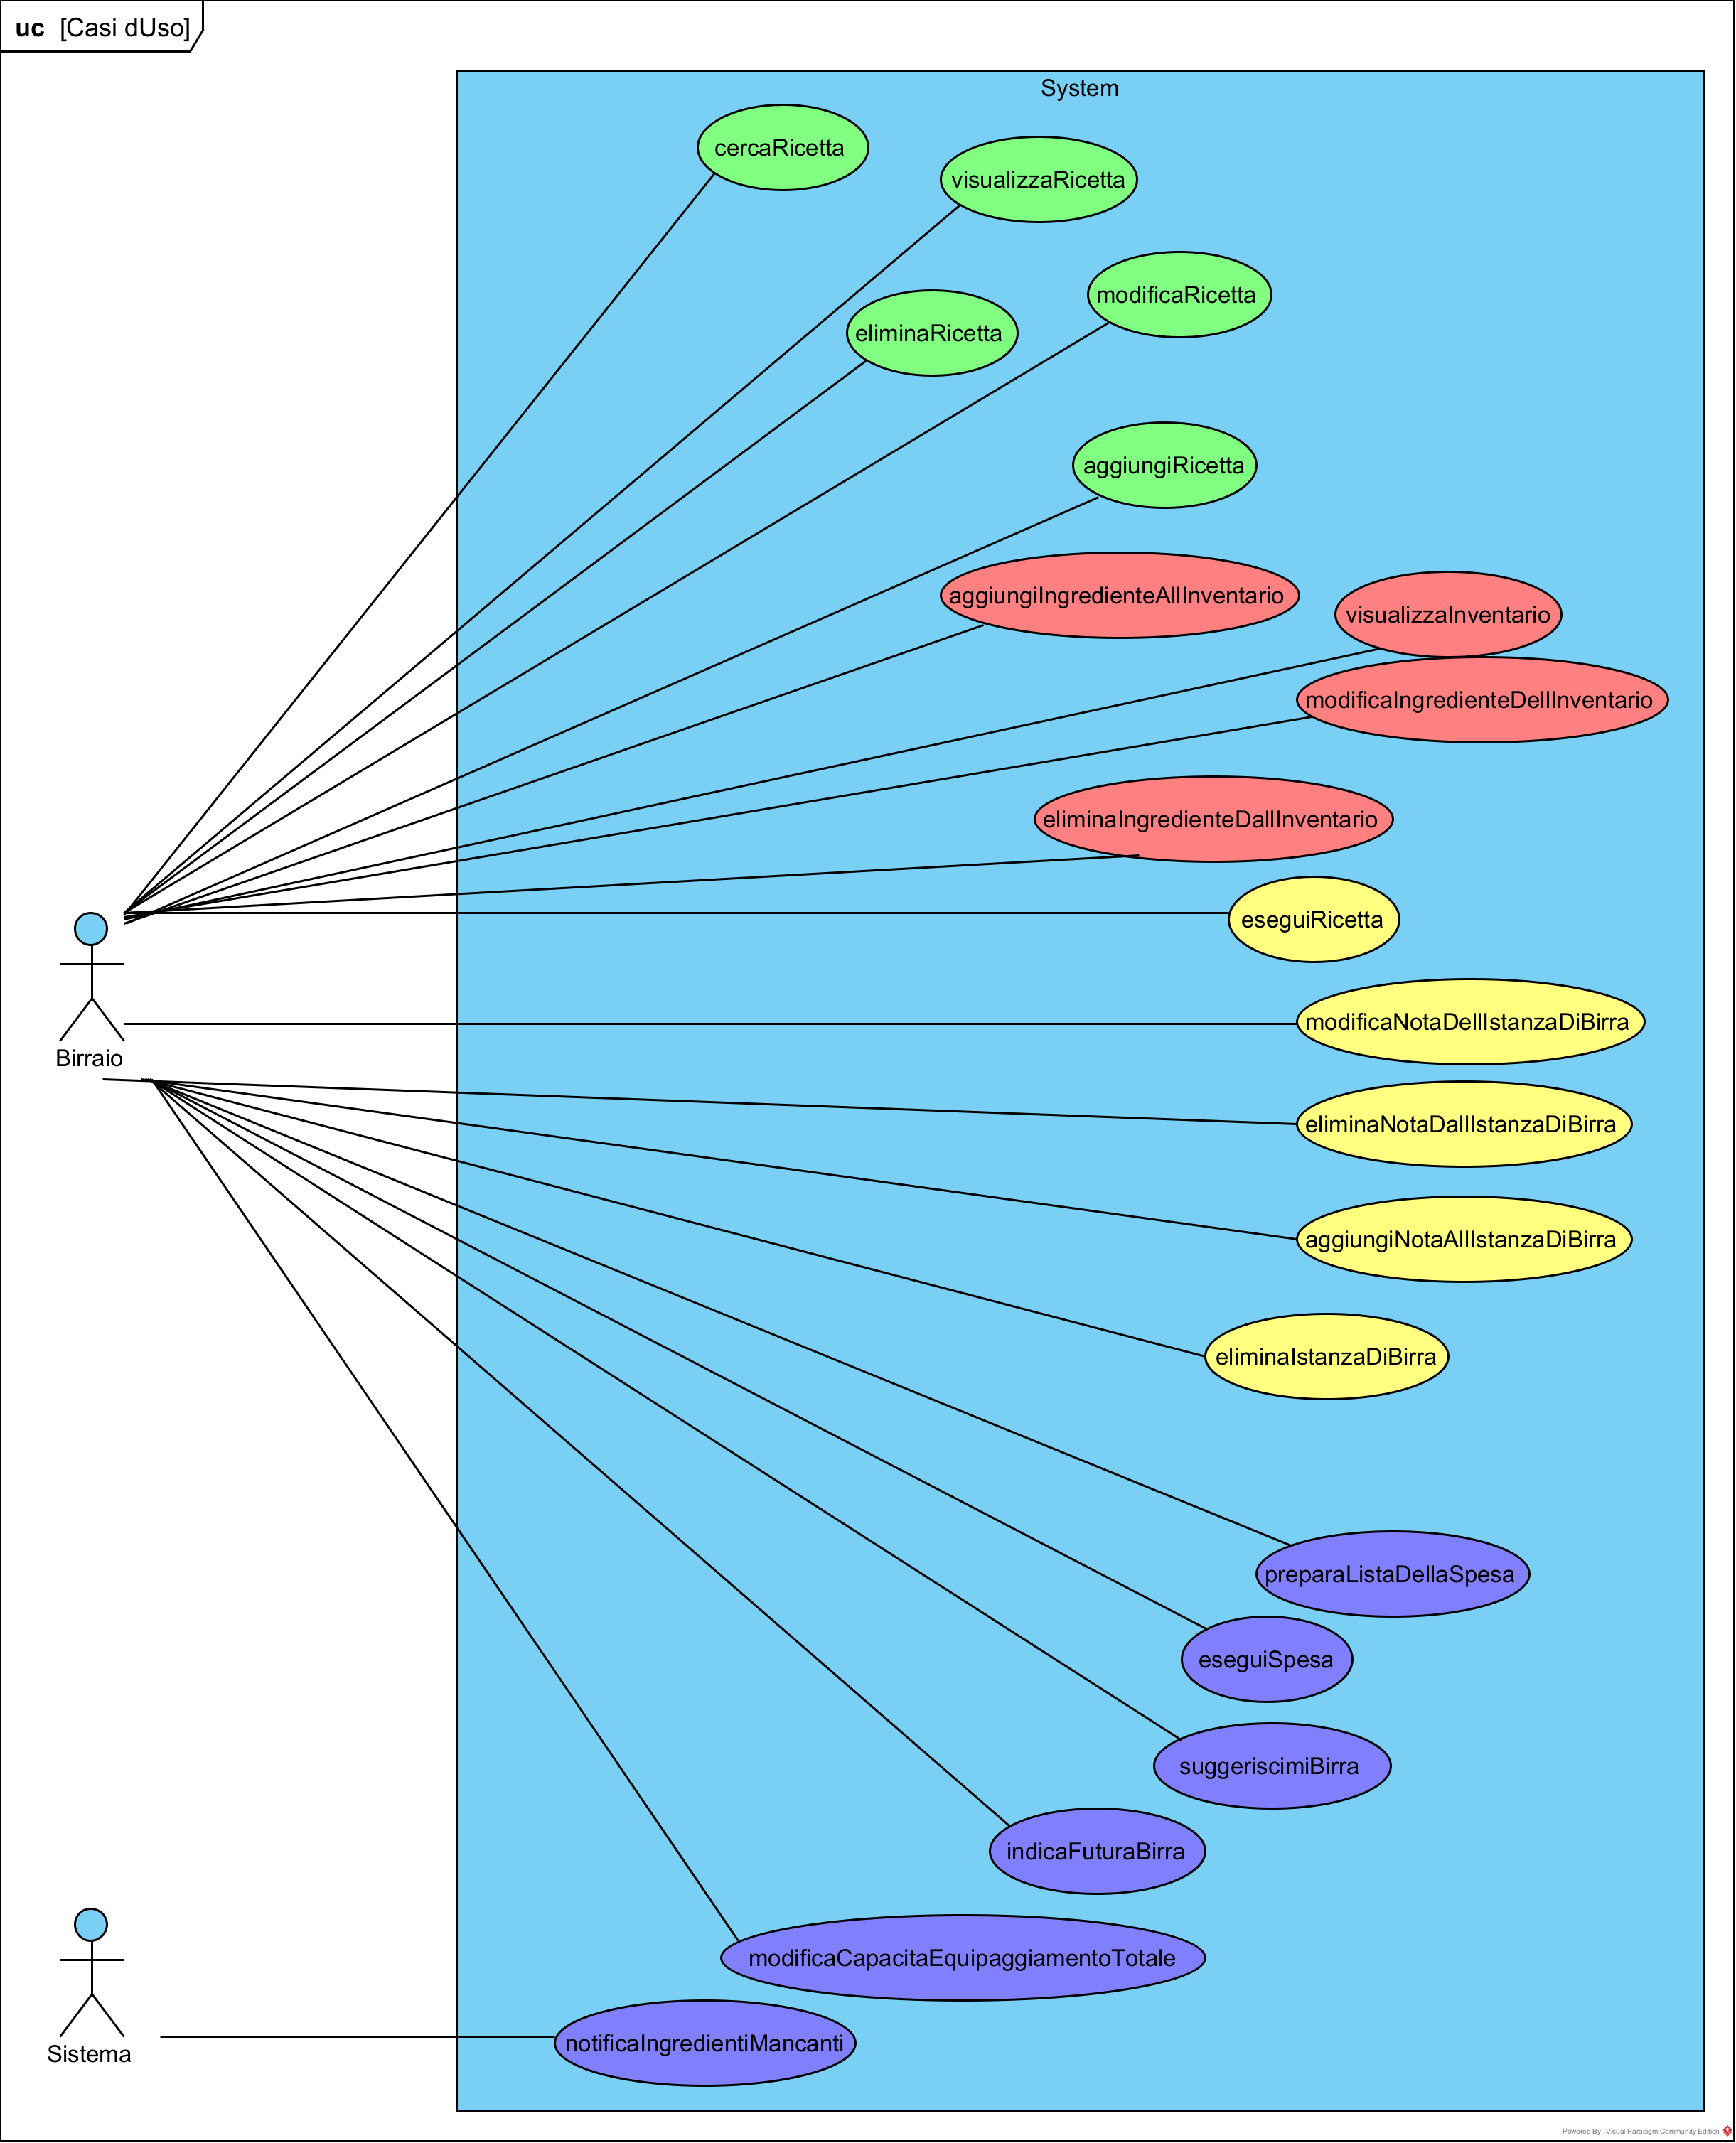
\includegraphics[width=1\linewidth]{image/Casi-dUso.png}
			\caption{Casi d'Uso}\label{fig:1}
		\end{figure}

		\subsection{Casi d'Uso in ogni iterazione}
			Abbiamo individuato i seguenti casi d'Uso suddivisi nelle 4 iterazioni svolte
			\begin{enumerate}
    				\item Prima Iterazione
					\begin{itemize}
						\item aggiungiRicetta	
						\item modificaRicetta	
						\item eliminaRicetta	
						\item cercaRicetta	
						\item visualizzaRicetta	
						\item visualizzaInventario	
						\item aggiungiIngredienteAllInventario	
						\item modificaIngredienteNellInventario	
						\item eliminaIngredienteDallInventario
					\end{itemize}
    				\item Seconda Iterazione
					\begin{itemize}
						\item eseguiRicetta	
						\item eliminaIstanzaDiBirra	
						\item aggiungiNotaAllIstanzaDiBirra		
						\item eliminaNotaDallIstanzaDiBirra	
						\item modificaNotaDellIstanzaDiBirra		
					\end{itemize}			
    				\item Terza Iterazione
					\begin{itemize}
						\item eseguiSpesa	
						\item indicaFuturaBirra	
						\item preparaListaDellaSpesa	
						\item suggeriscimiBirra	
						\item notificaIngredientiMancanti	
						\item modificaCapacitaEquipaggiamentoTotale		
					\end{itemize}
				\item Quarta Iterazione - nessuno
			\end{enumerate}
		
		\subsection{Caso d'Uso in formato breve - aggiungiRicetta}
			\begin{enumerate}
    				\item Il birraio inizia l'immissione di una nuova ricetta.
    				\item Il birraio inserisce il nome della nuova ricetta.
				\item Il birraio può inserire una descrizione della ricetta.
    				\item import caso d'uso modificaRicetta
    				\item il sistema salva la ricetta		
			\end{enumerate}		
	
		\subsection{Caso d'Uso in formato breve - modificaRicetta}	
			\begin{enumerate}
    				\item Il birraio inizia la modifica di una ricetta.
    				\item while:
				\begin{enumerate}
					\item  if opt1:
						\begin{enumerate}
							\item inserisce il nome di un ingrediente
							\item inserisce la quantita' dell'ingrediente
						\end{enumerate}		
					\item  if opt2:
						\begin{enumerate}
							\item individua l'ingrediente da rinominare
							\item inserisce il nuovo nome dell'ingrediente
						\end{enumerate}		
					\item  if opt3:
						\begin{enumerate}
							\item individua un ingrediente
							\item inserisce la nuova quantita' dell'ingrediente
						\end{enumerate}
 					\item  if opt4:
						\begin{enumerate}
  							\item seleziona l'ingrediente da eliminare
						\end{enumerate}	
 					\item  if opt5:
						\begin{enumerate}
  							\item inserisce il nuovo nome della ricetta
						\end{enumerate}
 					\item  if opt6:
						\begin{enumerate}
  							\item inserisce la nuova descrizione della ricetta
						\end{enumerate}	
    					\item il sistema salva la ricetta
				\end{enumerate}	
			\end{enumerate}
			
	\newpage	
	\section{Modello di Dominio}
	
		\begin{figure}[!h]
			\centering
			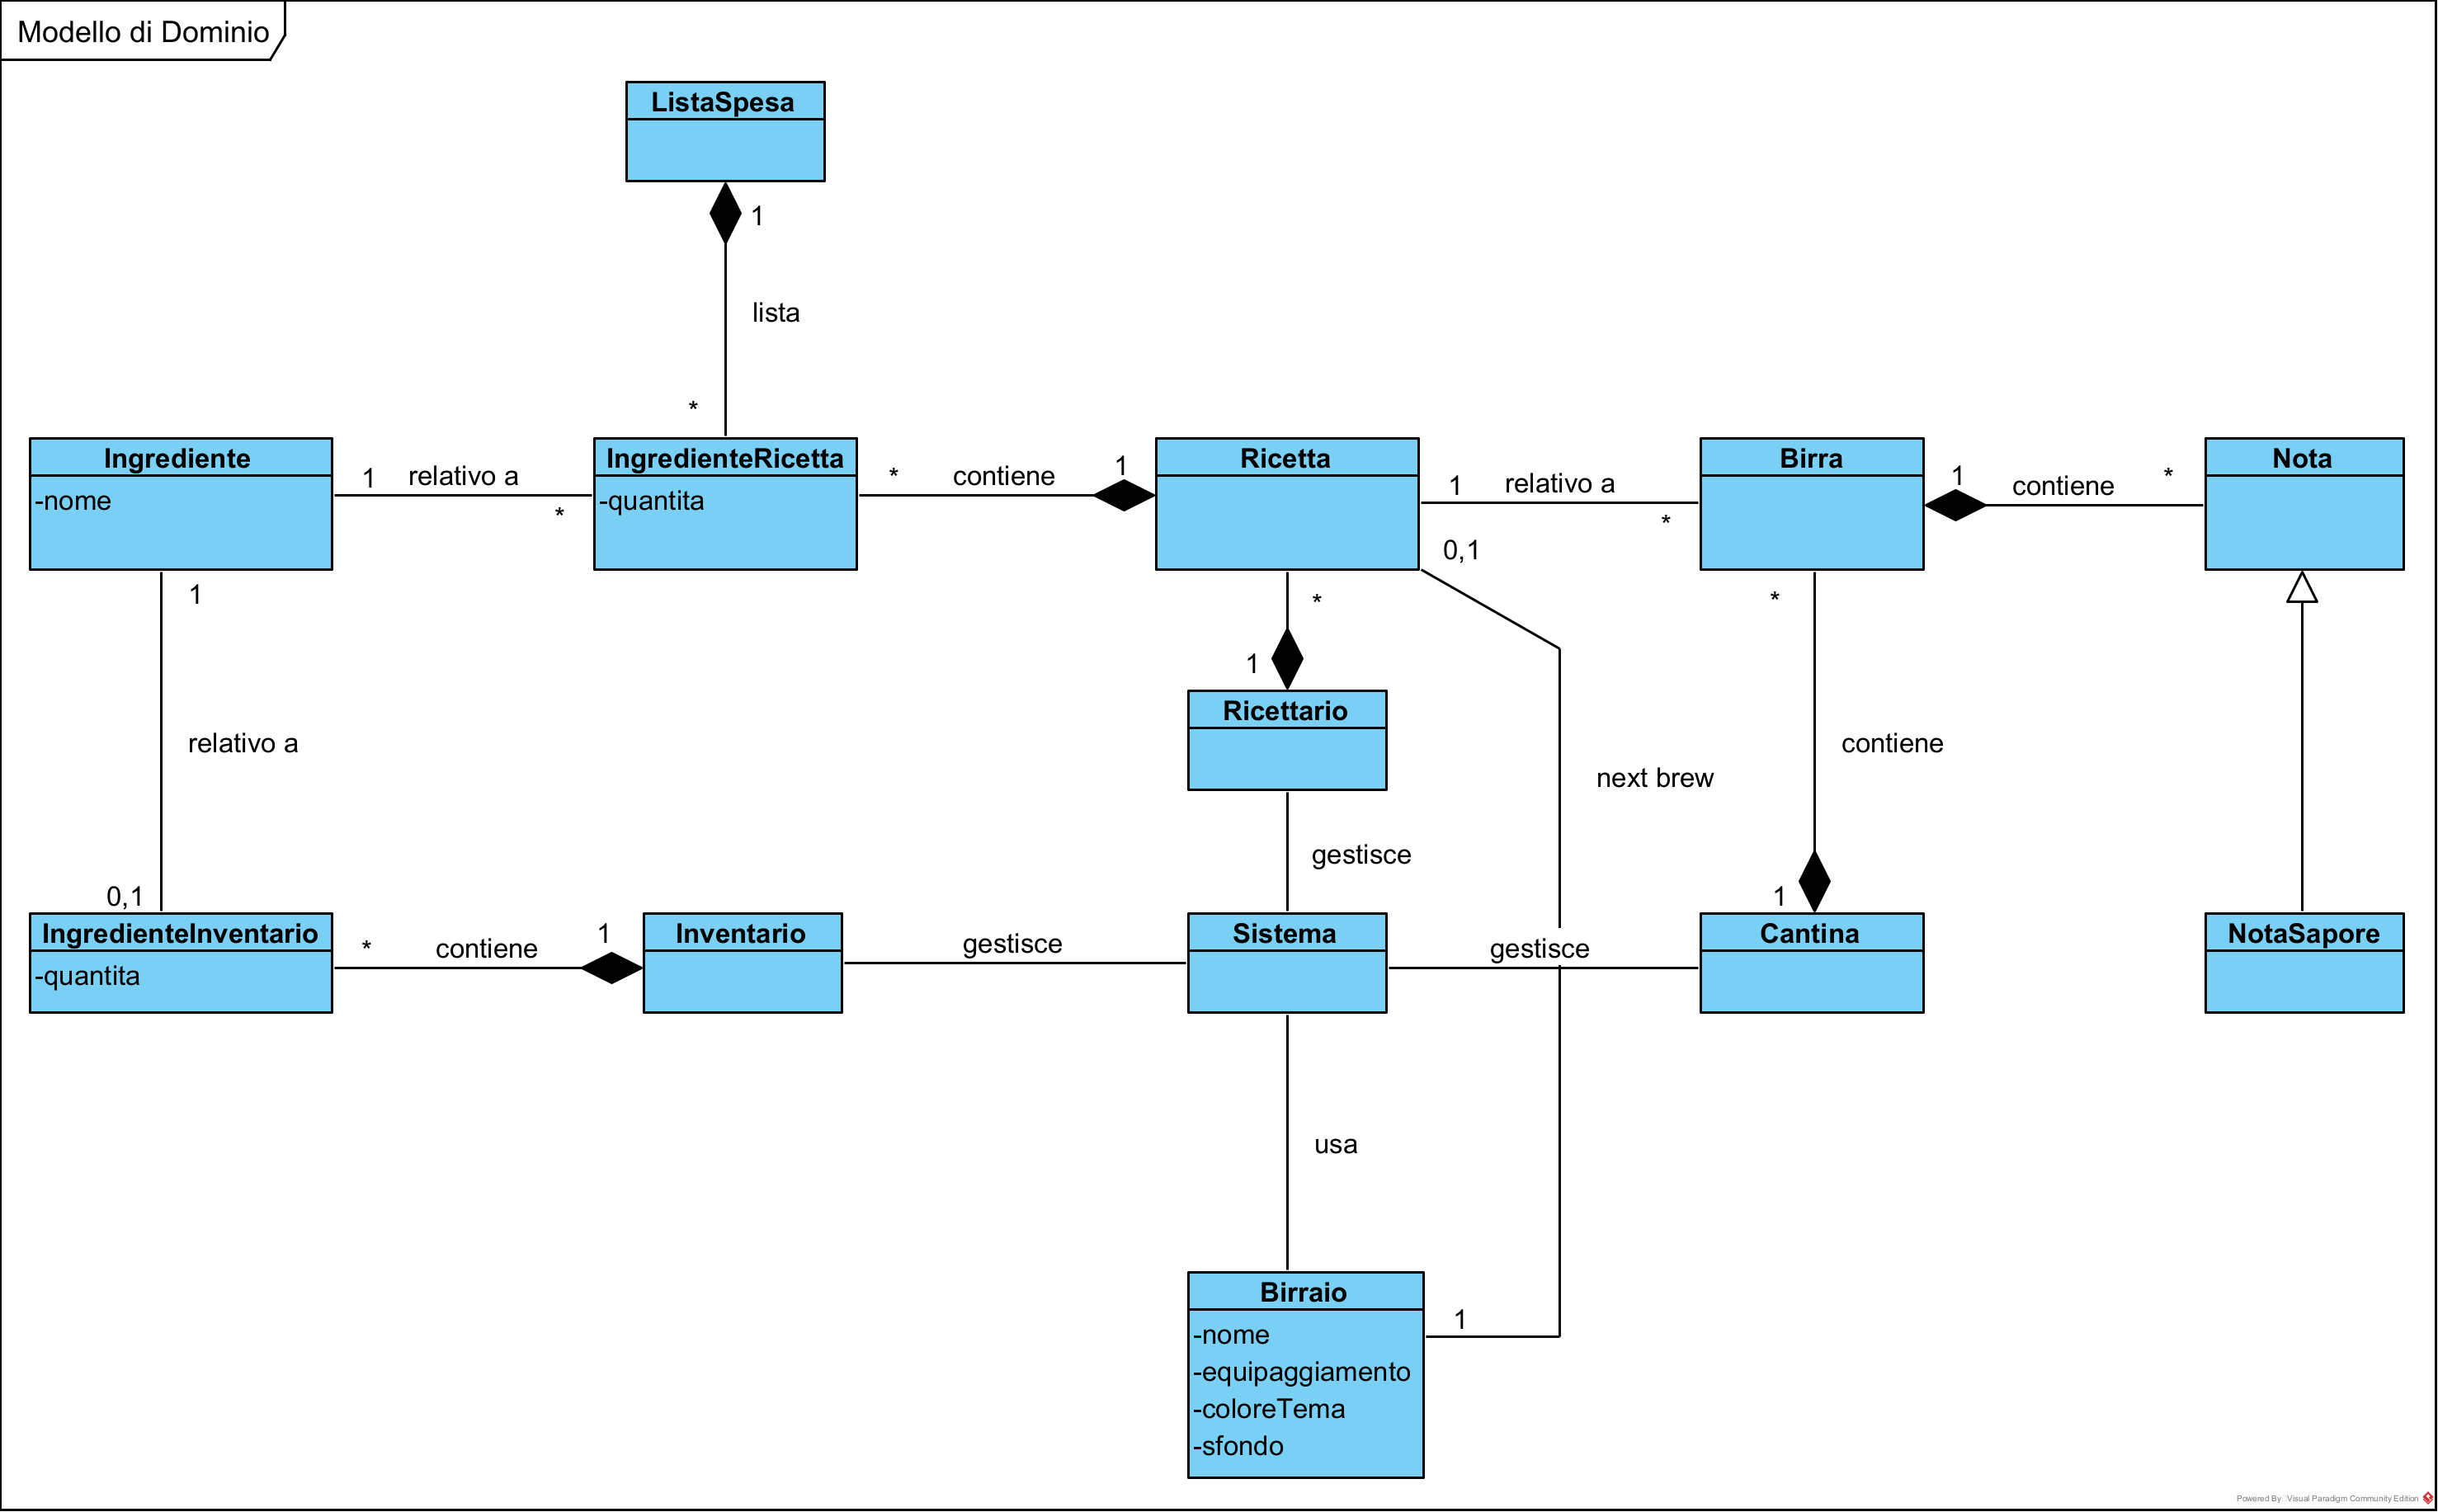
\includegraphics[width=1\linewidth]{image/Modello-di-Dominio.png}
			\caption{Casi d'Uso}\label{fig:1}
		\end{figure}

	\newpage
	\section{Diagrammi di Sequenza di Sistema}
	
		\subsection{SSD - aggiungiRicetta}
			\begin{figure}[!h]
				\centering
				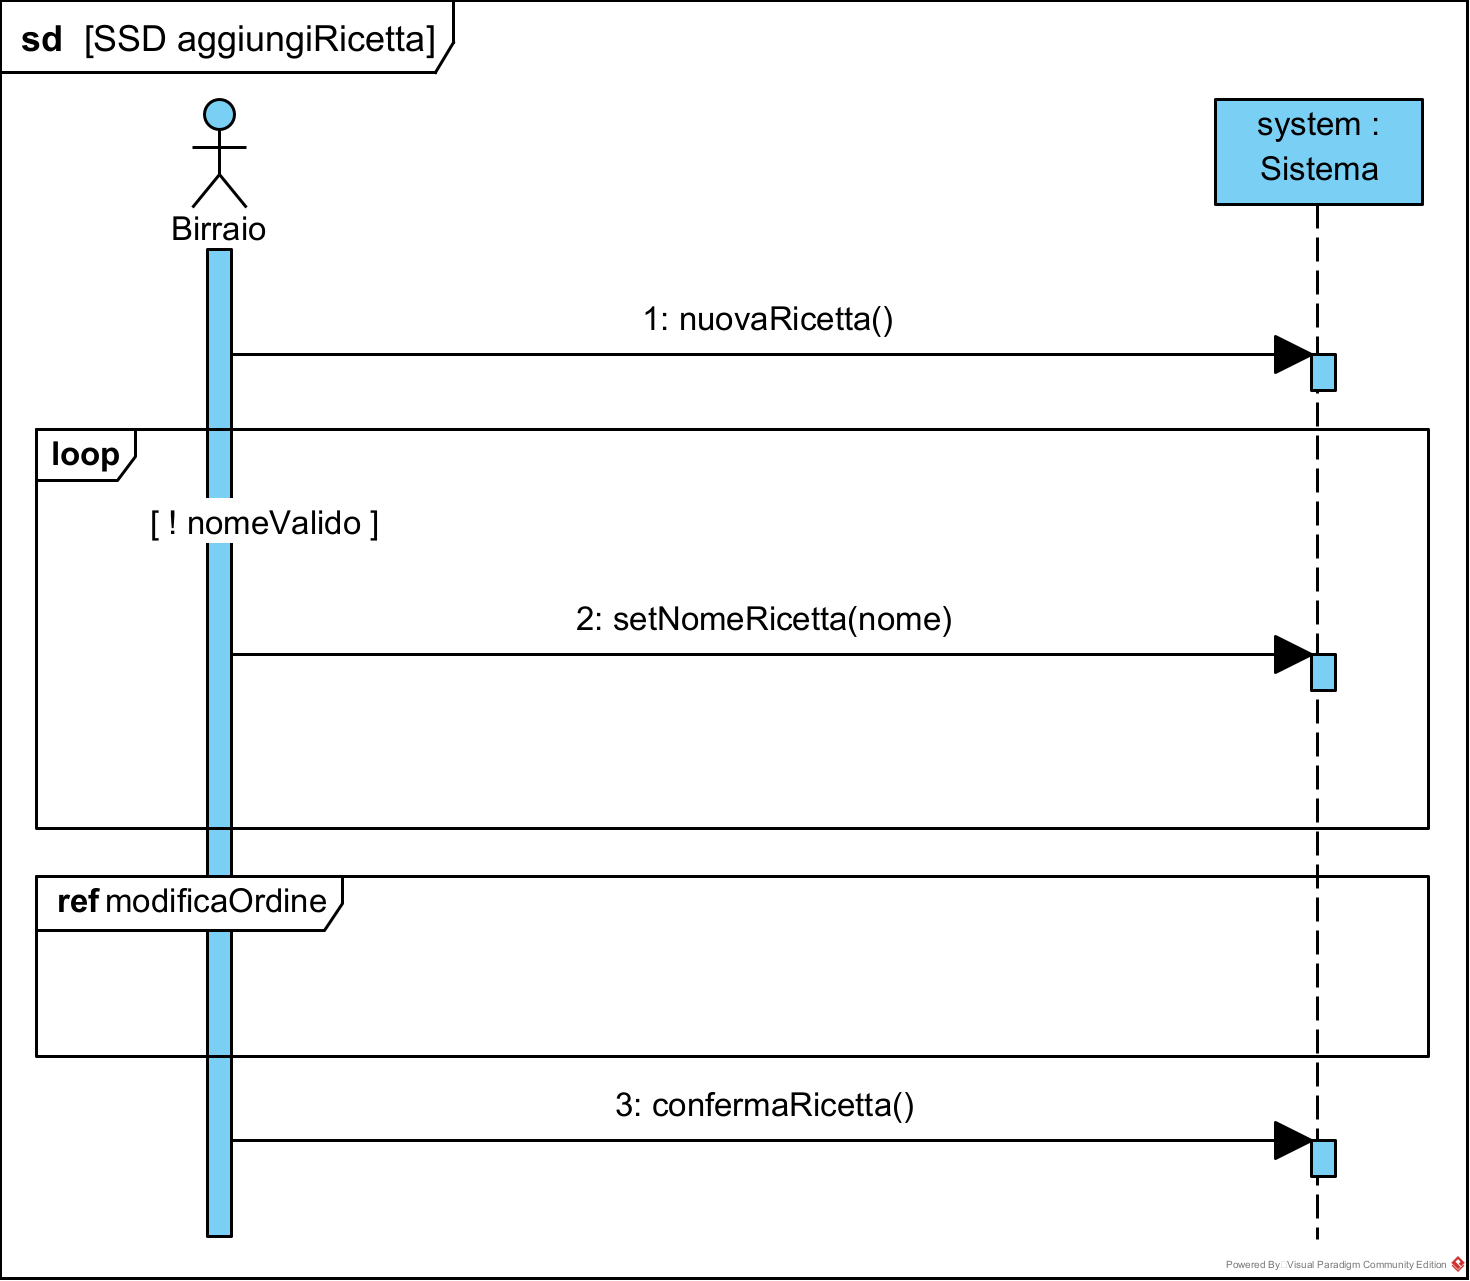
\includegraphics[width=0.8\linewidth]{image/SSD-aggiungiRicetta.png}
				\caption{SSD - aggiungiRicetta}\label{fig:1}
			\end{figure}	
		\newpage	
		\subsection{SSD - modificaRicetta}
			\begin{figure}[!h]
				\centering
				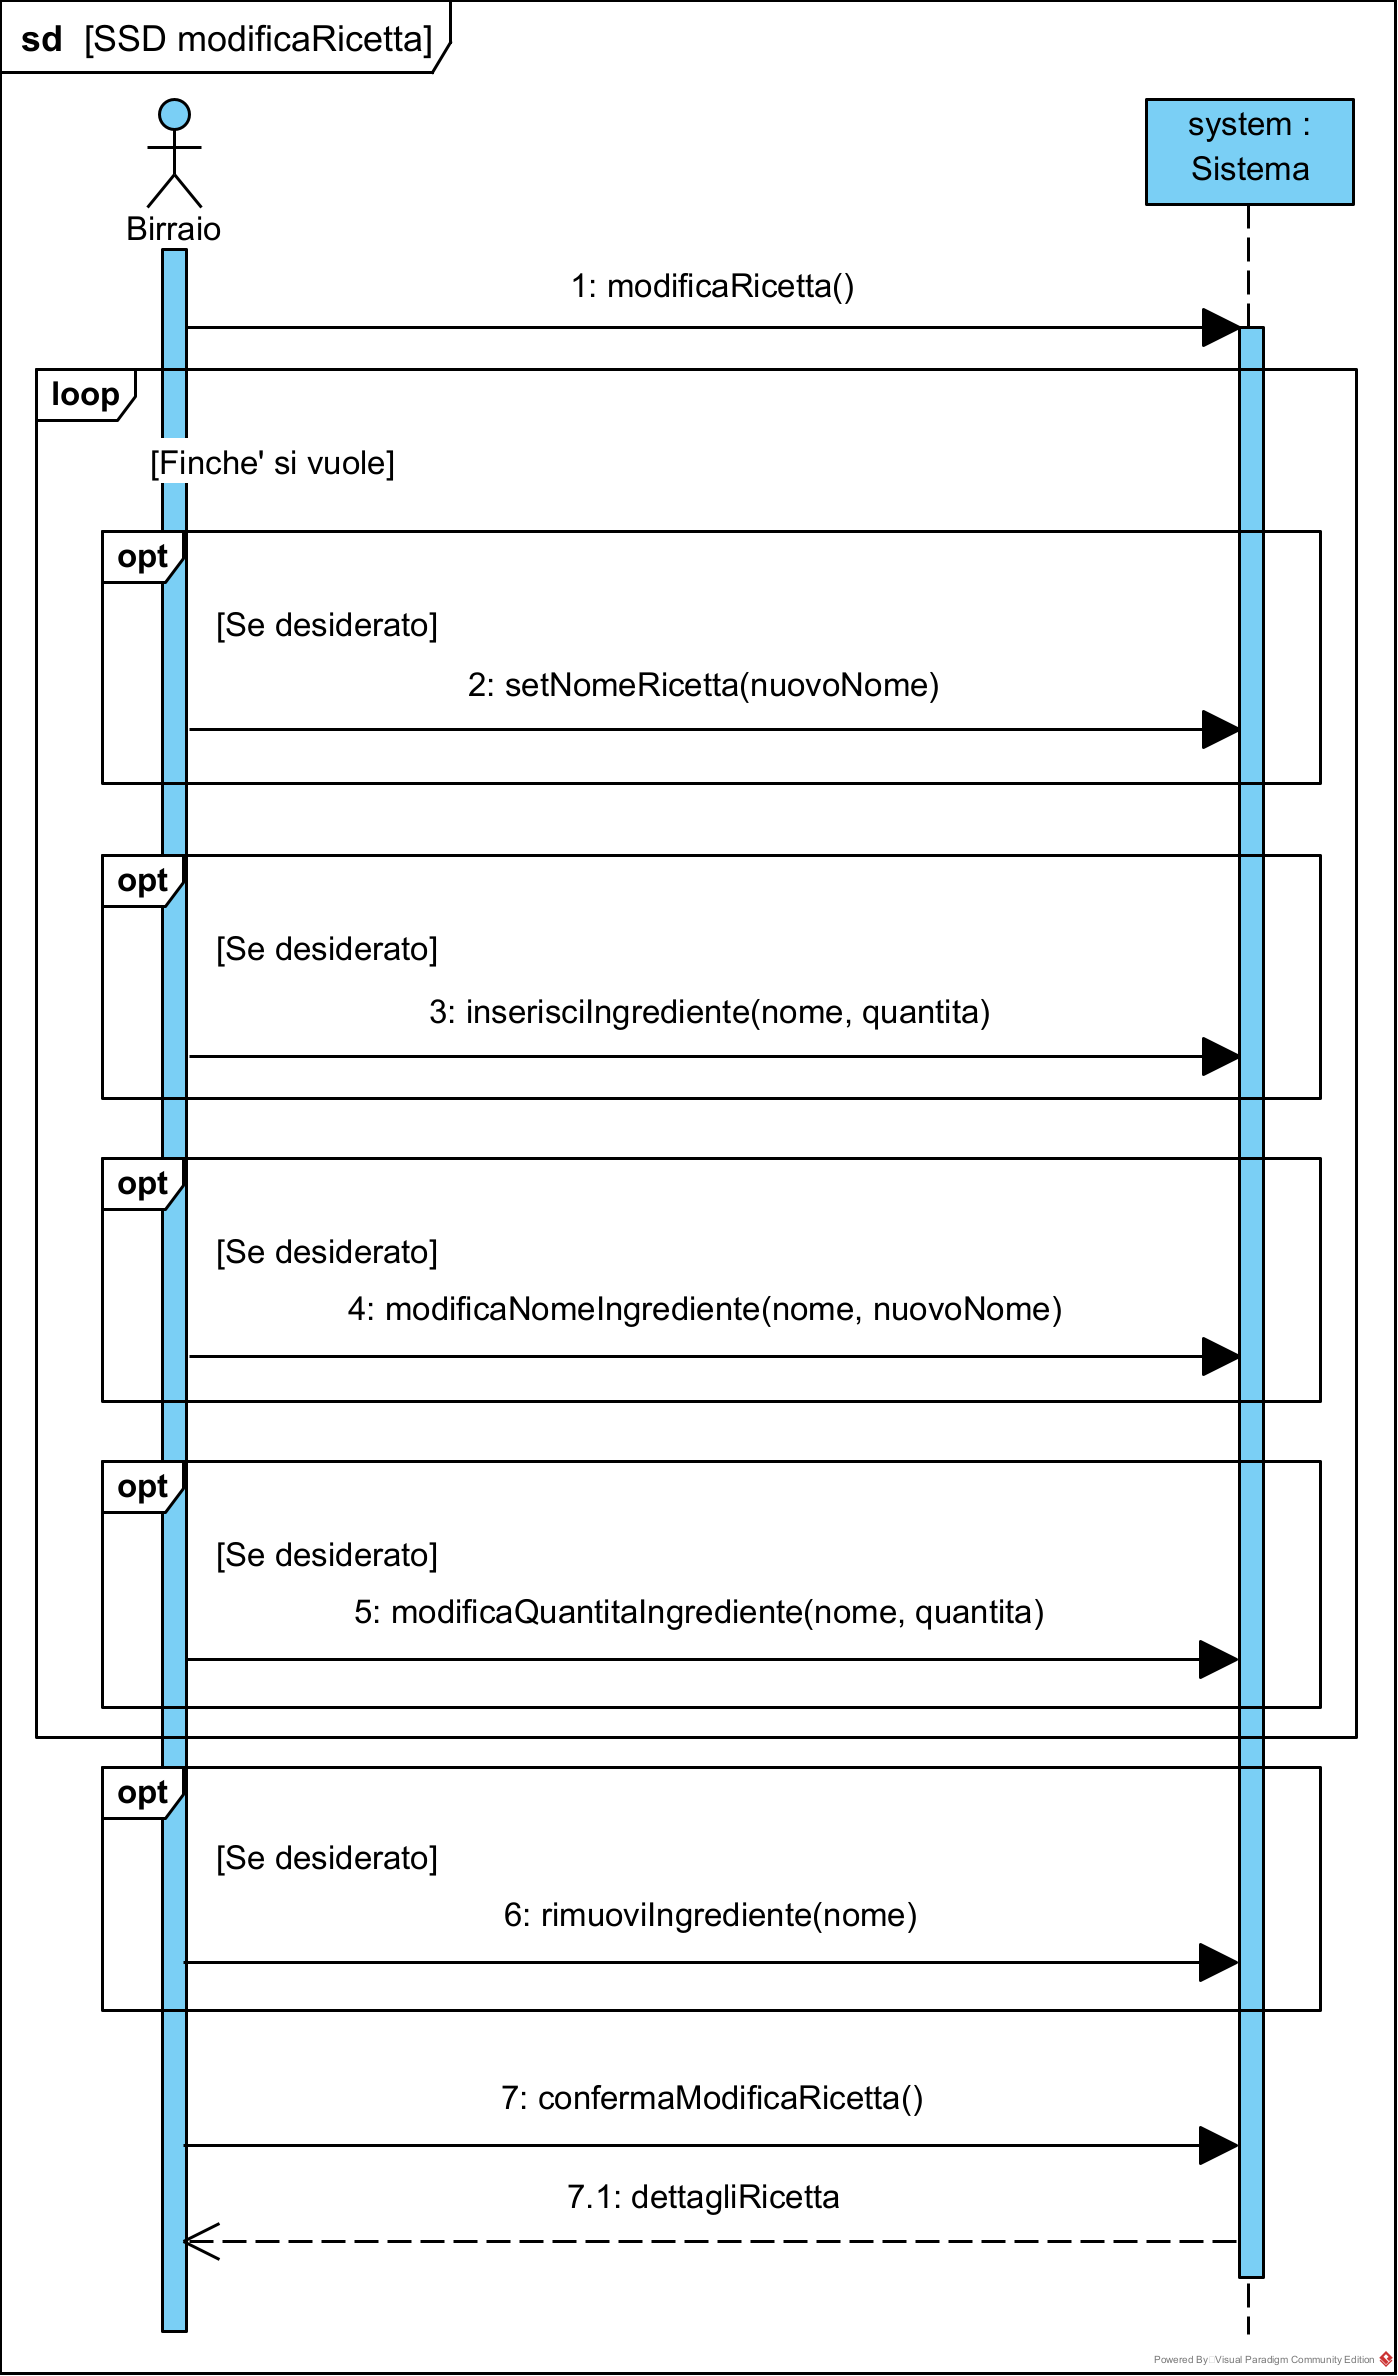
\includegraphics[width=0.8\linewidth]{image/SSD-modificaRicetta.png}
				\caption{SSD - modificaRicetta}\label{fig:1}
			\end{figure}


      \chapter{Progettazione}
         \section{Architettura del Sistema}
         \section{Diagramma delle Classi di Progettazione}
         
      	\section{Diagrammi di Sequenza}    
		\subsection{SD - modificaQuantitaIngrediente}
			\begin{figure}[!h]
				\centering
				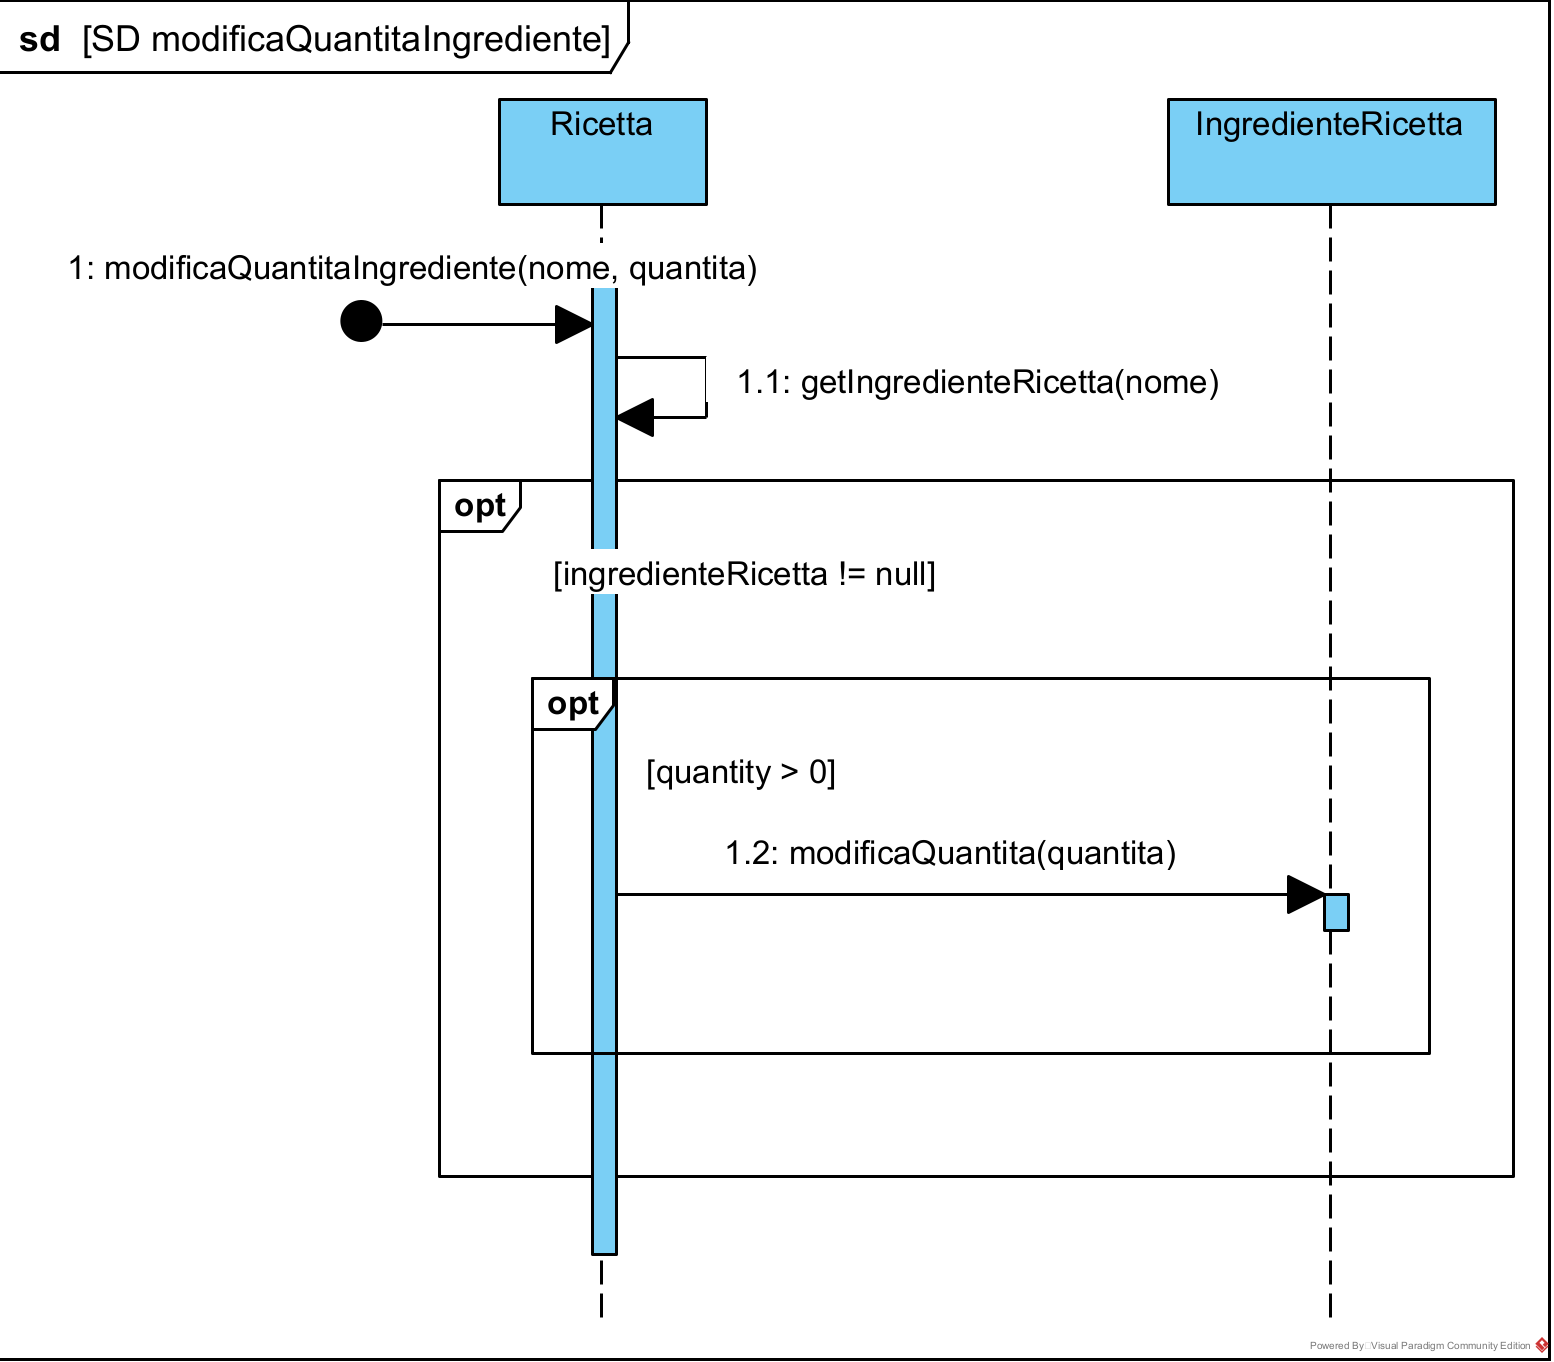
\includegraphics[width=0.7\linewidth]{image/SD-modificaQuantitaIngrediente.png}
				\caption{SD - modificaQuantitaIngrediente}\label{fig:1}
			\end{figure}	
		\newpage	
		\subsection{SD - modificaNomeIngrediente}
			\begin{figure}[!h]
				\centering
				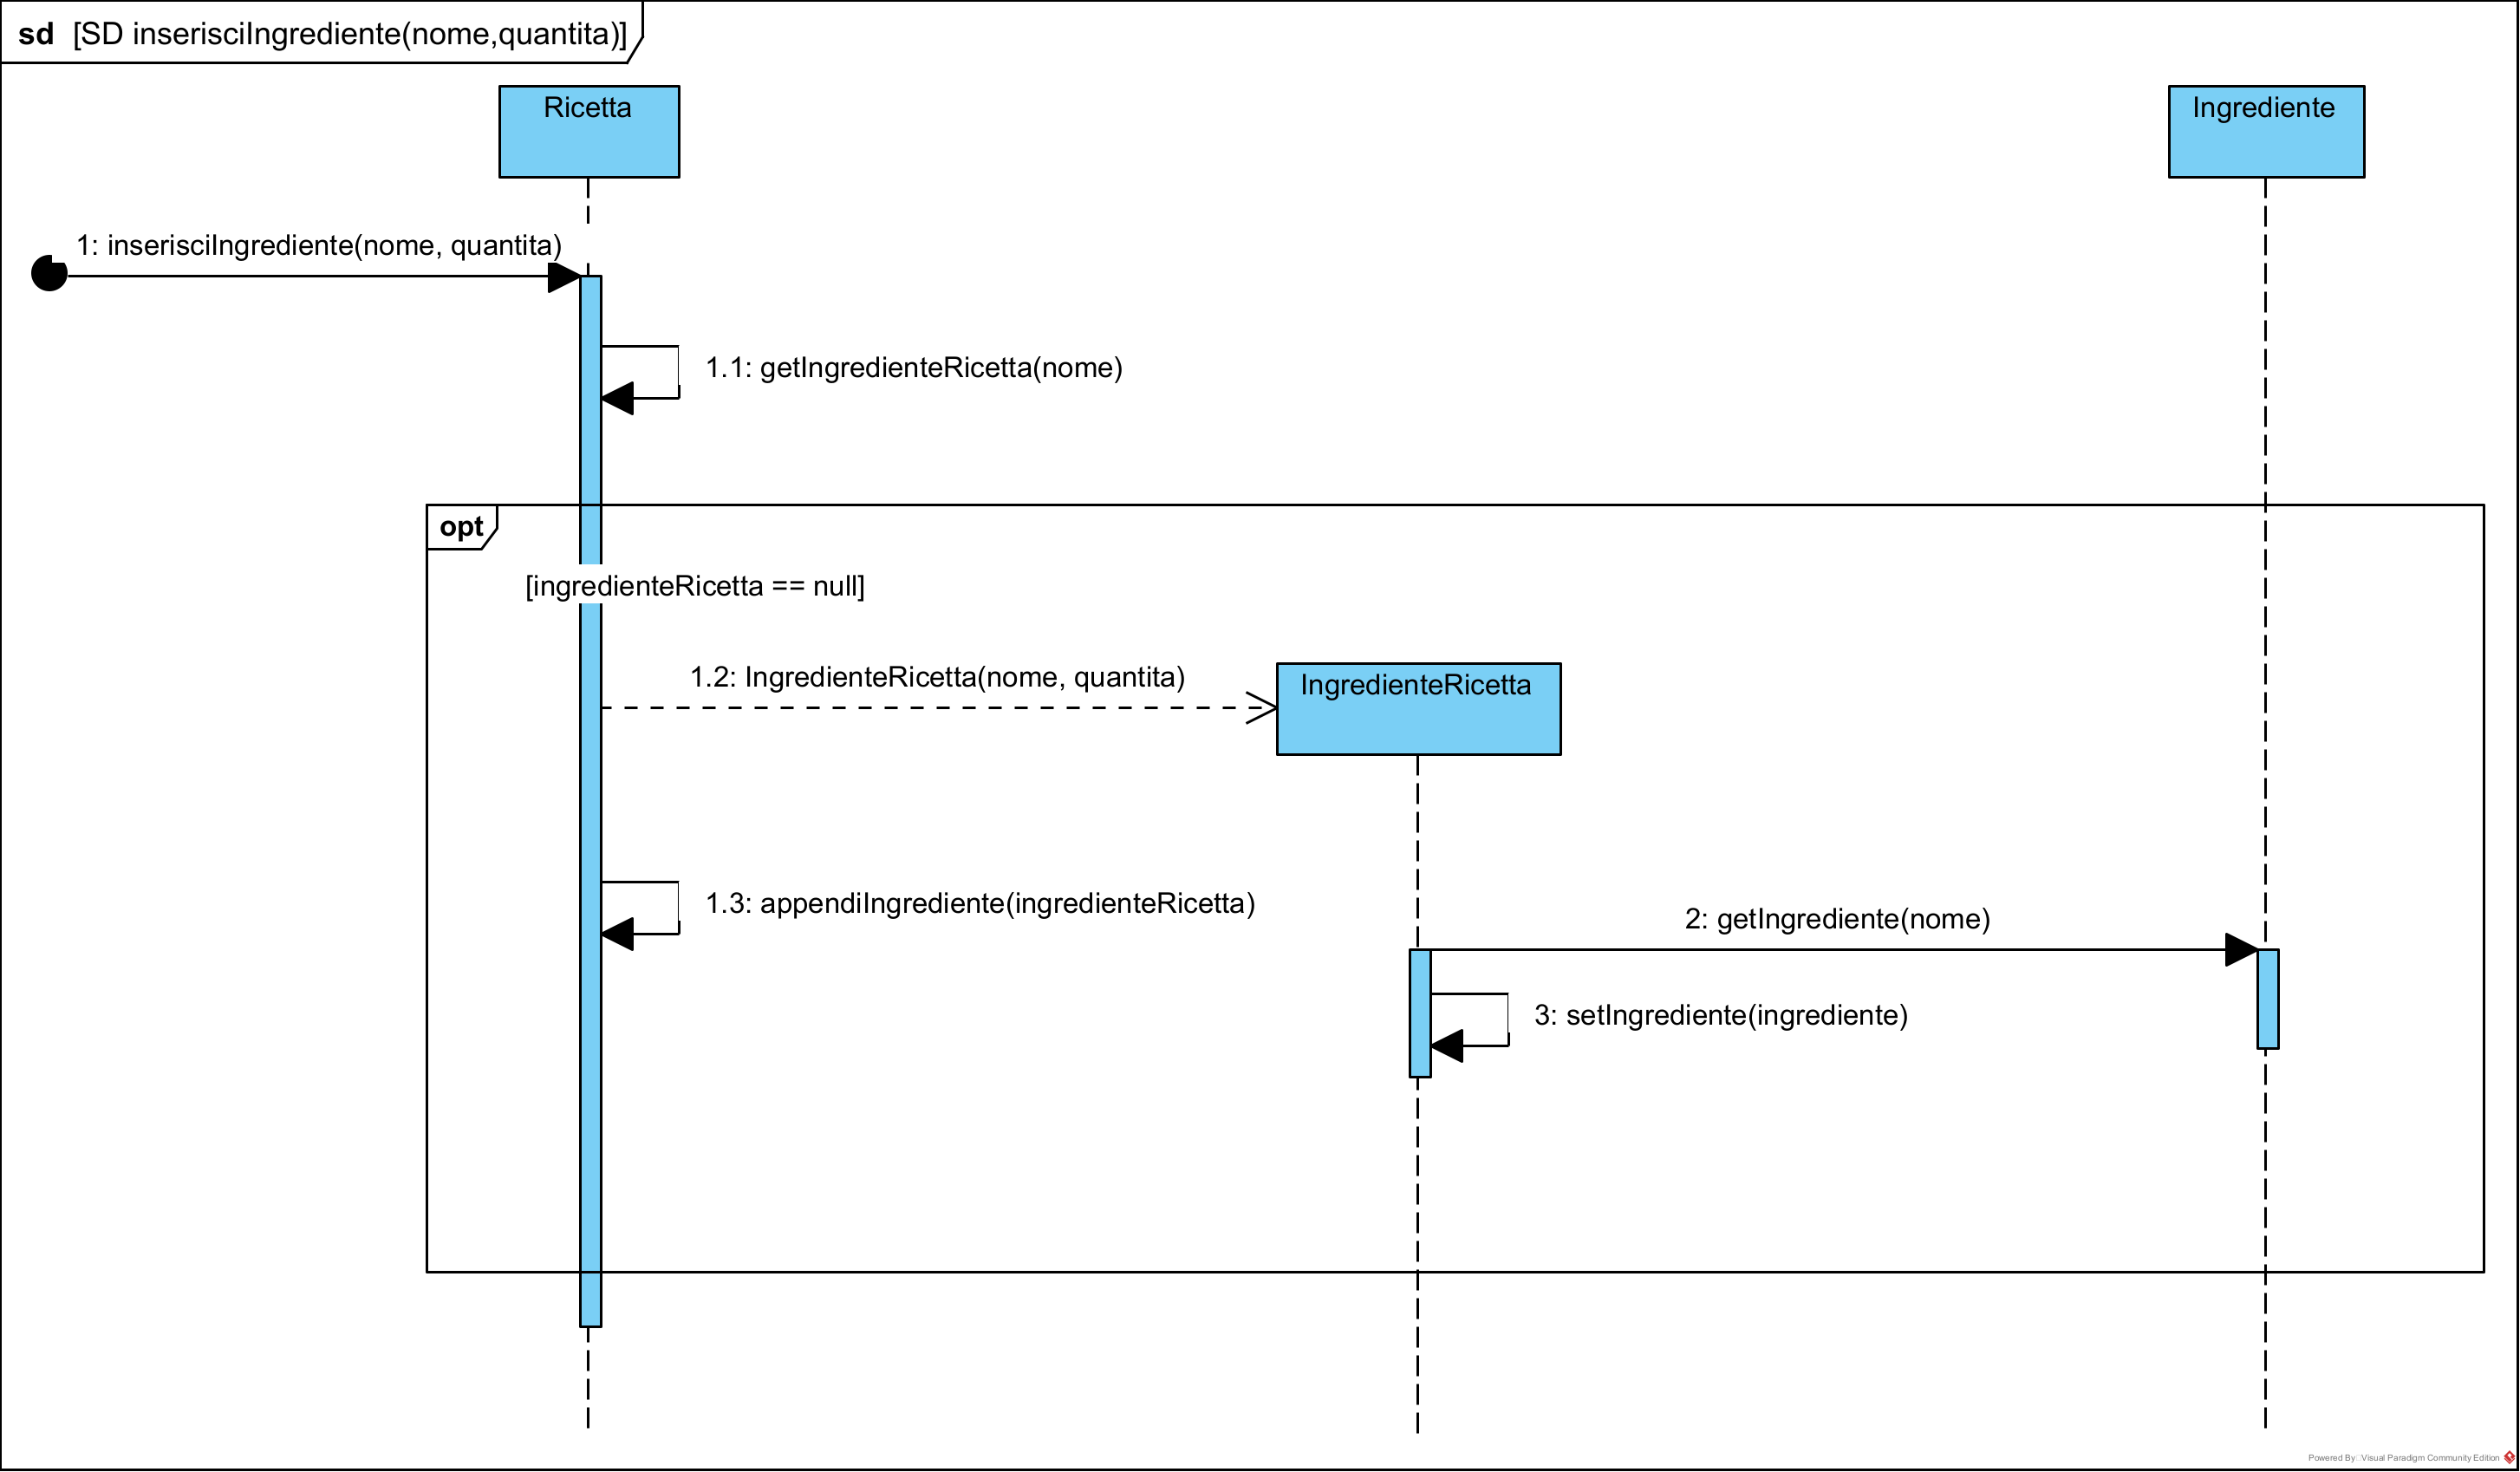
\includegraphics[width=0.8\linewidth]{image/SD-inserisciIngrediente.png}
				\caption{SD - inserisciIngrediente}\label{fig:1}
			\end{figure}
			
			
      \chapter{Conclusioni}
	commenti sull'esperianza
    
\end{document}
